41. $\cfrac{x^2-3x+2}{2x+3}\leqslant\cfrac{x^2-3x+2}{x+5}\Leftrightarrow (x^2-3x+2)\left(\cfrac{1}{2x+3}-\cfrac{1}{x+5}\right)\leqslant0
\Leftrightarrow (x^2-3x+2)\cdot\cfrac{x+5-2x-3}{(2x+3)(x+5)}\leqslant0\Leftrightarrow\cfrac{-(x-1)(x-2)^2}{(2x+3)(x+5)}\leqslant0.$ Применив метод интервалов, найдём ответ: $x\in\left(-5;-\cfrac{3}{2}\right)\cup[1;+\infty).$
\begin{figure}[ht!]
\center{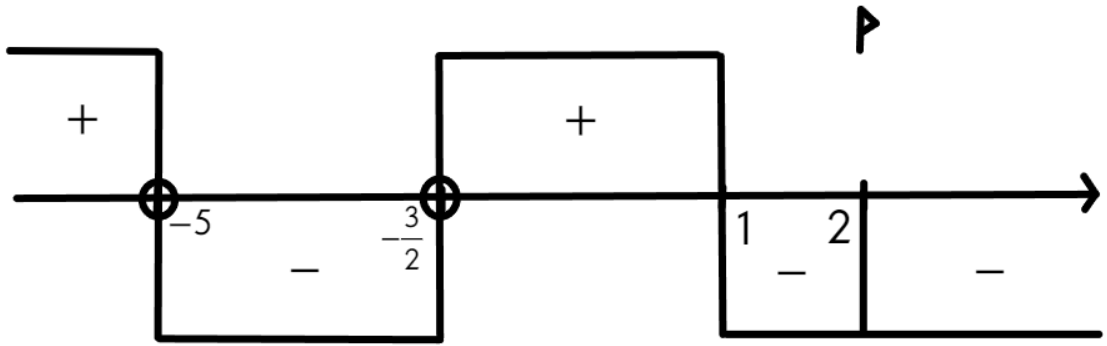
\includegraphics[scale=0.35]{ner9-41.png}}
\end{figure}\\
